%
% domain.tex -- Domain for problem 50000025
%
% (c) 2019 Prof Dr Andreas Müller, Hochschule Rapperswil
%
\documentclass[tikz,12pt]{standalone}
\usepackage{amsmath}
\usepackage{times}
\usepackage{txfonts}
\usepackage{pgfplots}
\usepackage{csvsimple}
\usetikzlibrary{arrows,intersections,math}
\begin{document}
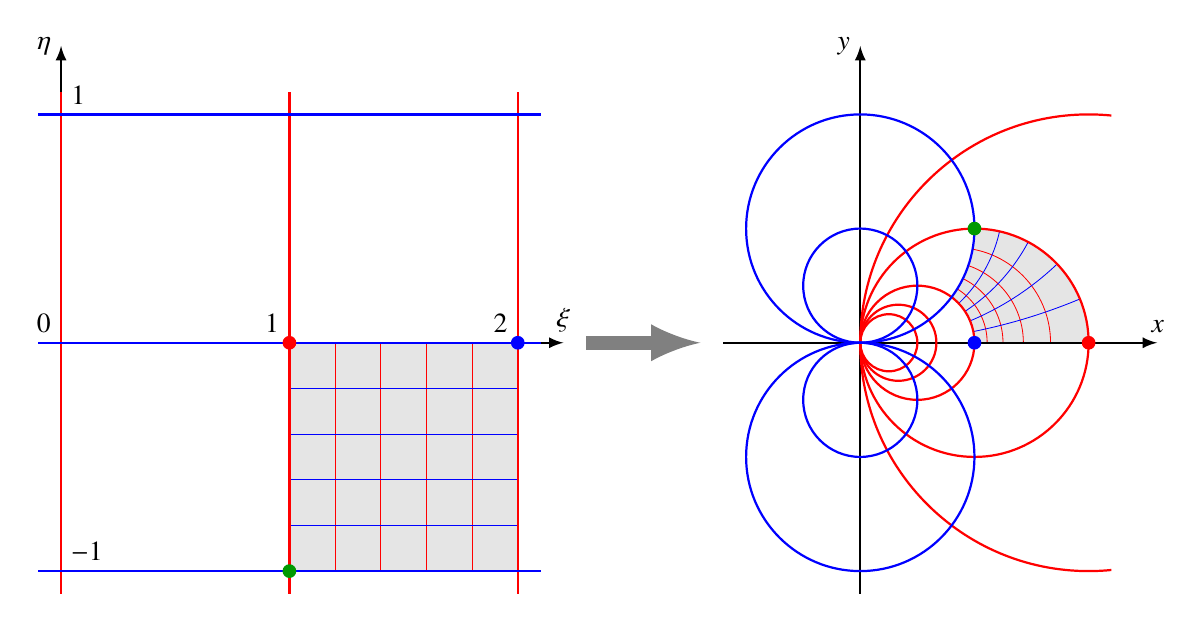
\begin{tikzpicture}[>=latex,thick,scale=2.9]

\definecolor{darkgreen}{rgb}{0,0.6,0}

\def\punkt#1#2{
	\fill[color=#2] #1 circle[radius=0.03];
}

\begin{scope}
	\fill[color=gray!20] (1,-1) rectangle (2,0);
	\foreach \a in {1.2,1.4,...,1.8}{
		\draw[color=red,line width=0.3pt] (\a,0) -- (\a,-1);
	}
	\foreach \b in {0.2,0.4,...,0.8}{
		\draw[color=blue,line width=0.3pt] (1,-\b) -- (2,-\b);
	}
	\draw[->] (-0.1,0) -- (2.2,0) coordinate[label=$\xi$];
	\draw[->] (0,-1.1) -- (0,1.3) coordinate[label={left:$\eta$}];
	\foreach \x in {0,1,2}{
		\draw[color=red] (\x,-1.1) -- (\x,1.1);
	}
	\foreach \y in {-1,0,1}{
		\draw[color=blue] (-0.1,\y) -- (2.1,\y);
	}
	\punkt{(1,0)}{red}
	\punkt{(2,0)}{blue}
	\punkt{(1,-1)}{darkgreen}
	\node at (0,0) [above left] {$0$};
	\node at (1,0) [above left] {$1$};
	\node at (2,0) [above left] {$2$};
	\node at (0,1) [above right] {$1$};
	\node at (0,-1) [above right] {$-1$};
\end{scope}

\begin{scope}[xshift=3.50cm]
	\begin{scope}
		\clip (0,0) -- (1,0) arc (0:180:0.5) -- cycle;
		\fill[color=gray!20] (0.5,0) circle[radius=0.5];
		\foreach \a in {1.2,1.4,...,2}{
			\draw[color=red,line width=0.3pt]
				({1/(2*\a)},0) circle[radius={1/(2*\a)}];
		}
		\foreach \b in {0.2,0.4,...,0.8}{
			\draw[color=blue,line width=0.3pt]
				(0,{1/(2*\b)}) circle[radius={1/(2*\b)}];
		}
		\fill[color=white] (0,0.5) circle[radius=0.5];
		\fill[color=white] (0.25,0) circle[radius=0.25];
	\end{scope}
	\draw[->] (-0.6,0) -- (1.3,0) coordinate[label={$x$}];
	\draw[->] (0,-1.1) -- (0,1.3) coordinate[label={left:$y$}];
	\clip (-1.1,-1.1) rectangle (1.1,1.1);
	\foreach \a in {0.5,1,2,3,4}{
		\draw[color=red] ({1/(2*\a)},0) circle[radius={1/(2*\a)}];
	}
	\foreach \b in {1,2}{
		\draw[color=blue] (0,{1/(2*\b)}) circle[radius={1/(2*\b)}];
		\draw[color=blue] (0,{-1/(2*\b)}) circle[radius={1/(2*\b)}];
	}
	\punkt{(1,0)}{red}
	\punkt{(0.5,0)}{blue}
	\punkt{(0.5,0.5)}{darkgreen}
\end{scope}

\draw[->,line width=5pt,color=gray] (2.3,0) -- (2.8,0);

\end{tikzpicture}
\end{document}

